\documentclass[UTF8]{ctexart}
\usepackage{hyperref}
\usepackage{abstract}
\usepackage[margin=1in]{geometry}
\usepackage{graphicx}
\usepackage{gensymb}
\usepackage{float}
\usepackage{amsmath}
\usepackage{multirow}
\usepackage{listings}
\lstset{breaklines}  
\lstset{extendedchars=false}   
\lstset{language=C++, 
    identifierstyle=,
    basicstyle=\ttfamily,
    stringstyle=\ttfamily,
    showstringspaces=false,
    frame=shadowbox, 
    captionpos=b
}
\begin{document}

\title{电子设计比赛“魑魅魍魉”组报告}
\maketitle

\tableofcontents
\newpage
\section{队伍简介}
\textbf{队伍名称:}魑魅魍魉

\textbf{队伍成绩:}三十二强(通过初试)

\textbf{小车图片:}见附录
\section{小车及技术资料}
\subsection{所用模块和器件}
\textbf{小车所用器件:}
\begin{itemize}
\item 四驱车底板
\item 稳压模块
\item 1100mah电池
\item 红外避障模块
\item 面包板
\item LED
\item 电机驱动模块L298N
\item 杜邦线
\item STM32F103RCT6
\item Zigbee无线串口收发模块
\item 陀螺仪JY62
\end{itemize}
\textbf{调试所用器件:}
\begin{itemize}
\item TTL转串口
\item HC-05蓝牙模块
\item ST-LINK仿真器
\end{itemize}
\section{整体设计思路}
\subsection{小车组成(硬件)设计}
为了平衡和易于控制,我们采用了四轮车的设计,将两对电机固定于四驱车底板上,引出各个电机的驱动电压输入端以及编码器,单片机生成特定占空比的PWM波输入电机驱动模块,电机驱动模块进而根据接收到的信号,输出相应占空比的电压幅值为12V的PWM波,用来驱动电机运转。由于四个电机是相对独立的,通过设置各个电机对应PWM波的性质,就可以完成最基本的四轮驱动。

为了让小车根据周围环境和上位机提供的信息,做出下一步行进的判断,所以还需要加入传感器,我们添加了红外传感器、Zigbee以及陀螺仪,其中,Zigbee直接与上位机交流,通过调用zigbee库中的函数,获取病人、医院、物资的位置信息,陀螺仪可以获得小车转角的信息,用于转弯和控制直行,而红外传感用于获得场内黑线的信息,用于辅助陀螺仪进行控制,另外上面提到利用霍尔效应的编码器,每次车轮转过一个确定的角度,会返回一个脉冲,所以可以反映小车车轮的转速和行进距离,也是一个重要的传感器,用于形成闭环,从而可以采用PID算法,不断调控小车自身,防止出现较大偏差。

以上是硬件方面,我们的全部设计思路,考虑到公平性,我们没有采用赛事方提供物资之外的材料。

\subsection{程序设计——模块化的设计}
总体的函数实现,有一个根本性的原则就是模块化,这样才便于调试和维护。(下面介绍本次比赛中最核心的几个模块化函数)
\subsubsection{基本的模块化函数}

    1.角度获取函数angle:利用陀螺仪获取小车角度。其函数如下:
    \begin{lstlisting}
        float angle()
        {
           static unsigned char ucRxBuffer[250];
           float a;
           int i=0;
           HAL_UART_Receive(&huart1,(uint8_t *)ucRxBuffer,20,0xFFFF);
           for(i=0;i<250;i++)
           {
              if(ucRxBuffer[i]==0x55&&ucRxBuffer[i+1]==0x53)
              {	
                 a=((short)(ucRxBuffer[i+7]<<8|ucRxBuffer[i+6]))/32768.0*180;
              }
            }
            return a;
        }
        \end{lstlisting}
   
        2.距离获取函数bip:利用stm32cubemx中的多线程对编码器的脉冲数进行积分,得出小车移动路程。其函数如下:
    \begin{lstlisting}
        Bip=0;
        int a=0,b=0;
        
        for(;;)
        {
           b=a;
           a=HAL_GPIO_ReadPin(GPIOA,GPIO_PIN_11);
           if(a!=b)
           {
             Bip+=1;
           }		
        }
        \end{lstlisting}
    
        3.四个小轮的单独驱动程序:单个轮子的函数接受的是0-1000的整数,对应0-100$\%$的占空比,如果是正数,则单个轮子前进,如是负数,那么单个轮子后退,下面展示的是右前轮的驱动函数,其他三个轮子与之相仿:
    \begin{lstlisting}
        void RightF(int value)
        {
            if(value>0)
            {
                __HAL_TIM_SetCompare(&htim2,TIM_CHANNEL_1,value);
                __HAL_TIM_SetCompare(&htim2,TIM_CHANNEL_2,0);
            }
            else
            {
                __HAL_TIM_SetCompare(&htim2,TIM_CHANNEL_1,0);
                __HAL_TIM_SetCompare(&htim2,TIM_CHANNEL_2,-value);
            }
        }
        \end{lstlisting}

    至此我们可以获得小车目前所在位置以及小车每一个轮子的转速,从而可以获得任何的行走方式。

\subsubsection{小车行进的实现——pid算法的使用}
将四个轮子单独的运行函数进一步打包,可以得到行进和转弯函数,如下:
\begin{lstlisting}
float Forward(float i1,float i2)
{
	RightB((int)(i1*800+i2*200));
	RightF((int)(i1*800+i2*200));
	LeftB((int)(i1*800-i2*200));
	LeftF((int)(i1*800-i2*200));
}

void Turn(float m)
{
	RightB(m*800);
	RightF(m*800);
	LeftB(-m*800);
	LeftF(-m*800);
}
\end{lstlisting}

PID函数接收小车目前角度和距离,也就是基础函数angle和bip的返回值,返回对于小车的控制值i1,i2和m。其中i1控制直行速度,i2用于行进过程中调节保持直行,m用于调控转弯速度。三个PID函数分别用于行进给定距离,转弯,保持直行,其内容如下:
\begin{lstlisting}
    float PIDturn(float error_sum1,float now1,float aim1)//转弯
    {
        float error,error_last,output1;
        error=now1-aim1;
        output1=error+error_sum1+(error-error_last);
        error_sum1=++error;
        if(error>45)
           error=45;
        if(error<-45)
           error=-45;
        error_last=error;
        return output1;
    }
    
    float PIDforward(float error_sum2,float now2,float aim2)//保持直行
    {
        int error,error_last;
        float output2;
        error=now2-aim2;
        output2=1.0*error+1.0*error_sum2+1.0*(error-error_last);
        error_sum2=++error;
        error_last=error;
        return output2;
    }
    
    float PIDstop(int now3,int aim3)//行进给定距离
    {
        int error,error_last;
        float output3;
        error_sum3=0;
        now3=Bip;
        error=aim3-now3;
        output3=2.0*error/500+error_sum3*0.01/500+0.1*(error-error_last)/500;
        if(error>400)
           error=400;
        if(error_sum3>5000)
           error_sum3=5000;
        return output3;
    }
    \end{lstlisting}

    至此,我们已经利用PID算法实现了小车的直行、转弯与停止。之后只需给小车直行、转弯与停止的指令,小车便会按照给定的指令进行稳定的运动。
\subsubsection{小车行进路线的获取——迷宫算法}

根据上位机提供的物资、病人、医院位置,以及目前的小车位置,我们对资源点、病人点、医院点进行合理赋值,通过迷宫算法算出最近距离,加权求和算出最优路径,最终生成小车行进指令的函数名为HEART,通过字符型数组传递direction传递行进路线。指令字符串由“字母+数字”的序列对组成,字母有四个,为F、B、L、R,分别表示相对于比赛场地中的绝对坐标的前后左右,而后面紧跟的数字表示行进格数。决策函数具体内容如下:
\begin{lstlisting}
    int map[6][6][4] = {0}; //0为无障碍物,0U,1D,3L,4R
    int Road[6][6] = {0};   //0代表没走过,1代表走过,因为走过的说明之前更短就能到达,就不必继续了
    int Value[6][6] = {0};
    char operationTotal[30];
    char direction[30];
    int ui = 0;
    int u = 1;
    typedef struct node
    {
        struct node *last;
        char dir; //从上一节点到此节点的方向
        int x;
        int y;
        struct node *next;
    } Node;
    Node *NodeSon[4]; //0U,1D,2L,3R
    typedef struct queue
    {
        Node *front;
        Node *rear;
    } Queue;
    
    Queue *RoadFinder;
    Node *hospital;
    
    int getValue(int x, int y, int V)
    {
        Value[x][y] = V;
    }
    
    void InitializeQueue(Queue *pq, Node *start)
    {
        pq->front = start;
        pq->rear = start;
        pq->front->next = pq->rear;
    }
    
    void Roadzero()
    {
        for (int i = 0; i < 6; i++)
            for (int j = 0; j < 6; j++)
                Road[i][j] = 0;
    }
    
    bool EnQueue(Node *pnew, Queue *pq)
    {
        pnew->next = NULL;
        pq->rear->next = pnew;
        pq->rear = pnew;
        return true;
    }
    
    Node *DeQueue(Queue *pq)
    {
        Node *pt;
        pt = pq->front;
        if (pq->front != pq->rear)
            pq->front = pq->front->next;
        return pt;
    }
    
    void EmptyQueue(Node *start)
    {
        Node *node2;
        while (start->next != NULL)
        {
            node2 = start->next;
            if (start != hospital)
                free(start);
            start = node2;
        }
        free(RoadFinder);
    }
    void Emptymiddle(Node *start, Node *end)
    {
        Node *node2 = start;
        node2 = node2->next;
        while (node2 != NULL)
        {
            start = node2;
            node2 = start->next;
            if (start != hospital)
                free(start);
        }
        free(RoadFinder);
    }
    Node **CNB(Node *temp) // Create Node Branch
    {
        if (temp->x > 0 && map[temp->x][temp->y][0] == 0 && Road[(temp->x) - 1][temp->y] != 1) //向上能走且没走过
        {
            NodeSon[0] = (Node *)malloc(sizeof(Node));
            NodeSon[0]->last = temp;
            NodeSon[0]->dir = 'U';
            NodeSon[0]->x = (temp->x) - 1;
            NodeSon[0]->y = (temp->y);
            Road[temp->x - 1][temp->y] = 1;
        }
        else
        {
            NodeSon[0] = NULL;
        }
    
        if (temp->x < 5 && map[temp->x][temp->y][1] == 0 && Road[(temp->x) + 1][temp->y] != 1) //向下能走且没走过
        {
            NodeSon[1] = (Node *)malloc(sizeof(Node));
            NodeSon[1]->last = temp;
            NodeSon[1]->dir = 'D';
            NodeSon[1]->x = (temp->x) + 1;
            NodeSon[1]->y = (temp->y);
            Road[temp->x + 1][temp->y] = 1;
        }
        else
        {
            NodeSon[1] = NULL;
        }
    
        if (temp->y > 0 && map[temp->x][temp->y][2] == 0 && Road[temp->x][temp->y - 1] != 1) //向下能走且没走过
        {
            NodeSon[2] = (Node *)malloc(sizeof(Node));
            NodeSon[2]->last = temp;
            NodeSon[2]->dir = 'L';
            NodeSon[2]->x = temp->x;
            NodeSon[2]->y = temp->y - 1;
            Road[temp->x][temp->y - 1] = 1;
        }
        else
        {
            NodeSon[2] = NULL;
        }
    
        if (temp->y < 5 && map[temp->x][temp->y][3] == 0 && Road[temp->x][temp->y + 1] != 1) //向下能走且没走过
        {
            NodeSon[3] = (Node *)malloc(sizeof(Node));
            NodeSon[3]->last = temp;
            NodeSon[3]->dir = 'R';
            NodeSon[3]->x = temp->x;
            NodeSon[3]->y = temp->y + 1;
            Road[temp->x][temp->y + 1] = 1;
        }
        else
        {
            NodeSon[3] = NULL;
        }
        return NodeSon;
    }
    
    Node *Check(Node **next4mb, Node *end)
    {
        int i;
        for (i = 0; i < 4; i++)
        {
            if (next4mb[i] == NULL)
                continue;
            else
            {
                if (next4mb[i]->x == end->x && next4mb[i]->y == end->y)
                    break;
            }
        }
        if (i == 4)
            return NULL;
        else
            return next4mb[i];
    }
    
    int En4mbQueue(Node **next4mb, Queue *RoadFinder)
    {
        for (int i = 0; i < 4; i++)
        {
            if (next4mb[i] != NULL)
                EnQueue(next4mb[i], RoadFinder);
        }
        return 1;
    }
    int PrintRoad(Node *EndInQueue, int Printb) //Printb is 1 the Print
    {
        char operation[100];
        Node *nod1 = EndInQueue, *nod2;
        int i;
        for (i = 0; i < 100; i++)
        {
            nod2 = nod1->last;
            if (nod2 == NULL)
                break;
            if (Value[nod2->x][nod2->y] == 10 && Printb == 1)
                Value[nod2->x][nod2->y] = 0;
            operation[i] = nod1->dir;
            nod1 = nod2;
        }
        if (Printb == 1)
        {
            for (int m = i - 1; m >= 0; m--)
            {
                operationTotal[ui] = operation[m];
                ui++;
            }
        }
        return i; //共走了i步
    }
    int FindRoad(Node *start, Node *end)
    {
        Roadzero();
        Node *temp; //FIFO出来的节点
        Node *EndInQueue = NULL;
        RoadFinder = (Queue *)malloc(sizeof(Queue));
        InitializeQueue(RoadFinder, start);
        RoadFinder->front = start;
        while (EndInQueue == NULL)
        {
            temp = DeQueue(RoadFinder);
            Node **next4mb = CNB(temp); //找到4个temp的下一部分节点
            EndInQueue = Check(next4mb, end);
            En4mbQueue(next4mb, RoadFinder);
        }
        if (PrintRoad(EndInQueue, 1))
            return 1;
        else
            return 0;
    }
    int CalDistance(Node *start, Node *end)
    {
        Roadzero();
        RoadFinder = (Queue *)malloc(sizeof(Queue));
        Node *temp; //FIFO出来的节点
        Node *EndInQueue = NULL;
    
        InitializeQueue(RoadFinder, start);
        RoadFinder->front = start;
        while (EndInQueue == NULL)
        {
            temp = DeQueue(RoadFinder);
            Node **next4mb = CNB(temp); //找到4个temp的下一部分节点
            EndInQueue = Check(next4mb, end);
            En4mbQueue(next4mb, RoadFinder);
        }
        return PrintRoad(EndInQueue, 0);
    }
    Node *findtheclose(Node *start)
    {
    
        int l = 0;
        int distance[10];
        Node *head = (Node *)malloc(sizeof(Node));
        Node *temp1 = head;
        Node *temp2;
        for (int i = 0; i < 6; i++)
            for (int j = 0; j < 6; j++)
            {
                if (Value[i][j] > 0 && Value[i][j] < 15)
                {
                    temp1->x = i;
                    temp1->y = j;
                    if (Value[i][j] == 10)
                    {
                        distance[l] = CalDistance(start, temp1);
                        Emptymiddle(start, temp1);
                    }
                    else
                    {
                        distance[l] = CalDistance(start, temp1);
                        Emptymiddle(start, temp1);
                        temp1->last = NULL;
                        for (int m = 0; m < 6; m++)
                            for (int n = 0; n < 6; n++)
                                if (Value[m][n] == 25)
                                {
                                    hospital->x = m;
                                    hospital->y = n;
                                }
                        distance[l] += CalDistance(temp1, hospital);
                        distance[l] = distance[l] / 3;
                        Emptymiddle(start, temp1);
                    }
                    temp2 = temp1;
                    temp1 = (Node *)malloc(sizeof(Node));
                    temp2->next = temp1;
                    l++;
                } //共有0-l-1个有用节点(实质上有0——l个)和hospital节点
            }
        int i;
        int j;
        for (i = 0; i < l; i++)
        {
            for (j = 0; j < l; j++)
            {
                if (distance[i] <= distance[j])
                    continue;
                else
                    break;
            }
            if (j == l)
                break;
        }
        Node *good = head;
        for (j = 0; j < i; j++)
        {
            good = good->next;
        }
        Node *temp = head;
        Node *ml;
        for (int m = 0; m < l + 1; m++)
        {
            ml = temp->next;
            if (m != i)
                free(temp);
            temp = ml;
        }
        return good;
    }
    
    Node *generateRoad(Node *start)
    {
        start->last = NULL;
        Node *end = findtheclose(start);
        FindRoad(start, end);
        end->last = NULL;
        if (Value[end->x][end->y] == 5)
        {
            FindRoad(end, hospital);
            Value[hospital->x][hospital->y] = 0;
            Value[end->x][end->y] = 0;
            EmptyQueue(start);
            return hospital;
        }
        Value[end->x][end->y] = 0;
        EmptyQueue(start);
        return end;
    }
    void getmap()
    {
        map[0][0][3] = 1;
        map[0][1][2] = 1;
        map[1][3][3] = 1;
        map[1][4][2] = 1;
        map[1][1][1] = 1;
        map[2][1][0] = 1;
        map[3][4][3] = 1;
        map[3][5][2] = 1;
        map[3][3][1] = 1;
        map[4][3][0] = 1;
        map[4][1][3] = 1;
        map[4][2][2] = 1;
        map[4][4][1] = 1;
        map[5][4][0] = 1;
        map[5][4][3] = 1;
        map[5][5][2] = 1;
        map[3][1][3] = 1;
        map[3][2][2] = 1;
    }
    void ValueSet()
    {
        getValue(0, 2, 10); //到时候可能需要定时中断,定过程中断
        getValue(2, 4, 10);
        getValue(3, 0, 10);
        getValue(3, 4, 10);
        getValue(4, 5, 10);
        getValue(5, 2, 10);
        getValue(2, 2, 5);
        getValue(5, 0, 25);
    }
    
    void Roadtrans()
    {
        direction[0] = operationTotal[0];
        char reference = operationTotal[0];
        int l = 0;
        for (int i = 0; i < ui; i++)
        {
            if (operationTotal[i] == reference)
            {
                l++;
            }
            else
            {
                direction[u] = 48 + l;
                u++;
                direction[u] = operationTotal[i];
                reference = operationTotal[i];
                u++;
                l = 1;
            }
            if(i == ui-1)
            {
                direction[u] = l + 48;
                u++;
            }
        }
    }
    int HEART()
    {
        hospital = (Node *)malloc(sizeof(Node));
        getmap();
        ValueSet();
        Node *start;
        start = (Node *)malloc(sizeof(Node));
        scanf("%d%d", &start->x, &start->y);
        for (int i = 0; i < 3; i++)
            start = generateRoad(start);
        Roadtrans();
        free(start);
        free(hospital);
    }
    \end{lstlisting}
    
至此,在已知小车的目前位置以及上位机提供的信息时,就可以利用该决策函数生成小车的行进路线,并且已经实现了稳定的直行,转弯与停止。那么需要一个核心执行程序来处理决策函数的命令,同时调用已经打包好的各个行进函数使小车根据指令运行,其内容如下:
    \begin{lstlisting}
        char direction[30];
        void Run()
        {
            for(i=0; direction[i]!='\0'; i=i+2)
            {
                if(direction[i]=='L')
                {
                    int o,num=0;
                    o=(int)direction[i+1]-(int)'0';
                    aim1=90+A;
                    aim3=o*B;
                    float error_sum1=0.0,error_sum2=0.0,now1;
                    int error_sum3=0;
                    now1=angle();
                    for(; now1-aim1>0.5||now1-aim1<-0.5;)
                    {
                        now1=angle();
                        Turn(PIDturn(error_sum1,now1,aim1));
                    }
                    Bip=0;
                    aim2=90+A;
                    for(;;)
                    {
                        now2=angle();
                        now3=Bip;
                        RunForward(PIDstop(now3,aim3),PIDforward(error_sum2,now2,aim2));
                    }
                }
                if(direction[i]=='R')
                {
                    int o,num=0;
                    o=(int)direction[i+1]-(int)'0';
                    aim1=-90+A;
                    aim3=o*B;
                    float error_sum1=0.0,error_sum2=0.0,now1;
                    int error_sum3=0;
                    for(; now1-aim1>0.5||now1-aim1<-0.5;)
                    {
                        now1=angle();
                        Turn(PIDturn(error_sum1,now1,aim1));
                    }
                    bbip=Bip;
                    aim2=-90+A;
                    for(; num;)
                    {
                        now2=angle();
                        now3=bbip-Bip;
                        RunForward(PIDstop(error_sum3,now3,aim3),PIDforward(error_sum2,now2,aim2));
                    }
                }
                if(direction[i]=='F')
                {
                    int o,num=0;
                    o=(int)direction[i+1]-(int)'0';
                    aim1=A;
                    aim3=o*B;
                    float error_sum1=0.0,error_sum2=0.0,now1;
                    int error_sum3=0;
                    for(; now1-aim1>0.5||now1-aim1<-0.5;)
                    {
                        now1=angle();
                        Turn(PIDturn(error_sum1,now1,aim1));
                    }
                    bbip=Bip;
                    aim2=A;
                    for(; num;)
                    {
                        now2=angle();
                        now3=bbip-Bip;
                        RunForward(PIDstop(error_sum3,now3,aim3),PIDforward(error_sum2,now2,aim2));
                    }
                }
                if(direction[i]=='B')
                {
                    int o,num=0;
                    o=(int)direction[i+1]-(int)'0';
                    aim1=-A;
                    aim3=o*B;
                    float error_sum1=0.0,error_sum2=0.0,now1;
                    int error_sum3=0;
                    for(; now1-aim1>0.5||now1-aim1<-0.5;)
                    {
                        now1=angle();
                        Turn(PIDturn(error_sum1,now1,aim1));
                    }
                    bbip=Bip;
                    aim2=-A;
                    for(; num;)
                    {
                        now2=angle();
                        now3=bbip-Bip;
                        RunForward(PIDstop(error_sum3,now3,aim3),PIDforward(error_sum2,now2,aim2));
                    }
                }
                if(direction[i]=='\0')
                {
                    StopRightNow();
                }
            }
        }
        \end{lstlisting}

        至此,所有功能都以模块化的方式实现。
\subsubsection{亮点}

\begin{itemize}
\item 采用四轮驱动,最大限度地提升了小车的灵活度,同时小车整体比较对称,便于控制。
\item 模块化程序的设计,便于调试与维护。
\item 通过调试PID算法的参数,实现了稳定的直行与转弯以及急停功能。
\item 迷宫算法(递归回溯法)的运用:对一个包括有很多个结点,每个结点有若干个搜索分支的问题,把原问题分解为若干个子问题求解的算法;当搜索到某个结点发现无法再继续搜索下去时,就让搜索过程回溯(回退)到该节点的前一个结点,继续搜索该节点外的其他尚未搜索的分支;如果发现该结点无法再搜索下去,就让搜索过程回溯到这个结点的前一结点继续这样的搜索过程;这样的搜索过程一致进行到搜索到问题的解或者搜索完了全部可搜索分子没有解存在为止。
\item 多线程的运用,使得小车保证进行获取数据的各项程序运行的同时正常执行决策程序生成的命令。
\end{itemize}

\subsubsection{不足}

\begin{itemize}
\item 对于硬件的了解不够深入,只能使用stm32cubemx帮助我们辅助调试,而不能够从底层调试硬件实现想要的功能;成员们都还未学习数字电路相关课程,所以也很难设计自行设计PCB。
\item 决策函数的路线规划采用了迷宫算法计算距离以及对特定点赋值,最后加权求和,以此迭代多次的方式来计算最优方案。实际上忽略了小车转弯所消耗时间等一系列其他的实际因素,需要增加这些因素带来的影响;迭代了三次相当于小车考虑了未来三步的进程,有时可能不够充分;这一决策方法在某些特殊的点以及障碍分布的情况下并不能得出较好的行进方案,仍需改进。
\item 由于每过30秒,物资会刷新,临近刷新时间时小车的行进规划还没有处理得很好。
\item 由于比赛时间与期中考试时间冲突,导致进入比赛场地调参的部分没有进行,所以未能取得较好成绩。
\end{itemize}

\section{个人贡献以及参赛感想与建议}
\subsection{个人贡献}
\begin{itemize}
\item 张鸿琳:队长,负责小组分工规划、组织,各个部分都有深入贡献。
\item邓润涛:PID算法的实现与调试,核心执行程序的实现。
\item邓雲峰:小车基础框架的搭建和利用迷宫算法编写决策函数。
\item孙杨:小车基础框架的搭建和接线。
\end{itemize}
\subsection{参赛感想}

\textbf{邓润涛:}本次比赛的难度非常好,没有过于劝退,过程中的每个困难能给我们带来提高;但是没有一个总览全局的人,对于机器整体的搭建与调试的整体认知不到位,每一个部位做好了,但是将其拼凑调试好也是非常需要花时间的地方,对于一个项目要有整体把握,这是我这次比赛学到最多的地方。

\textbf{张鸿琳:}参与本次比赛,我学到了很多关于单片机的知识,从一个连面包板都不知道是什么的萌新逐渐开始自己动手接线,编程,构思,找BUG,越来越享受整个创造的过程。小车能够收到指令并正常运行的那一刻,我感受到的快乐与满足是前所未有的,也燃起了我极大的信心,未来也会更主动地参与到类似的赛事来挑战自己。同时,我还认识了一群志同道合的朋友,一起为了相同的目标爆肝,制作小车时我们还受到了学长通俗易懂的细致指导,他们时刻关注着我们的进展,也为我们的进步感到高兴,这些都是我难以忘怀的宝贵经历,感谢这次比赛带给我的知识与历练。


\section{附录:小车图片}
\begin{figure}[H]
\centering
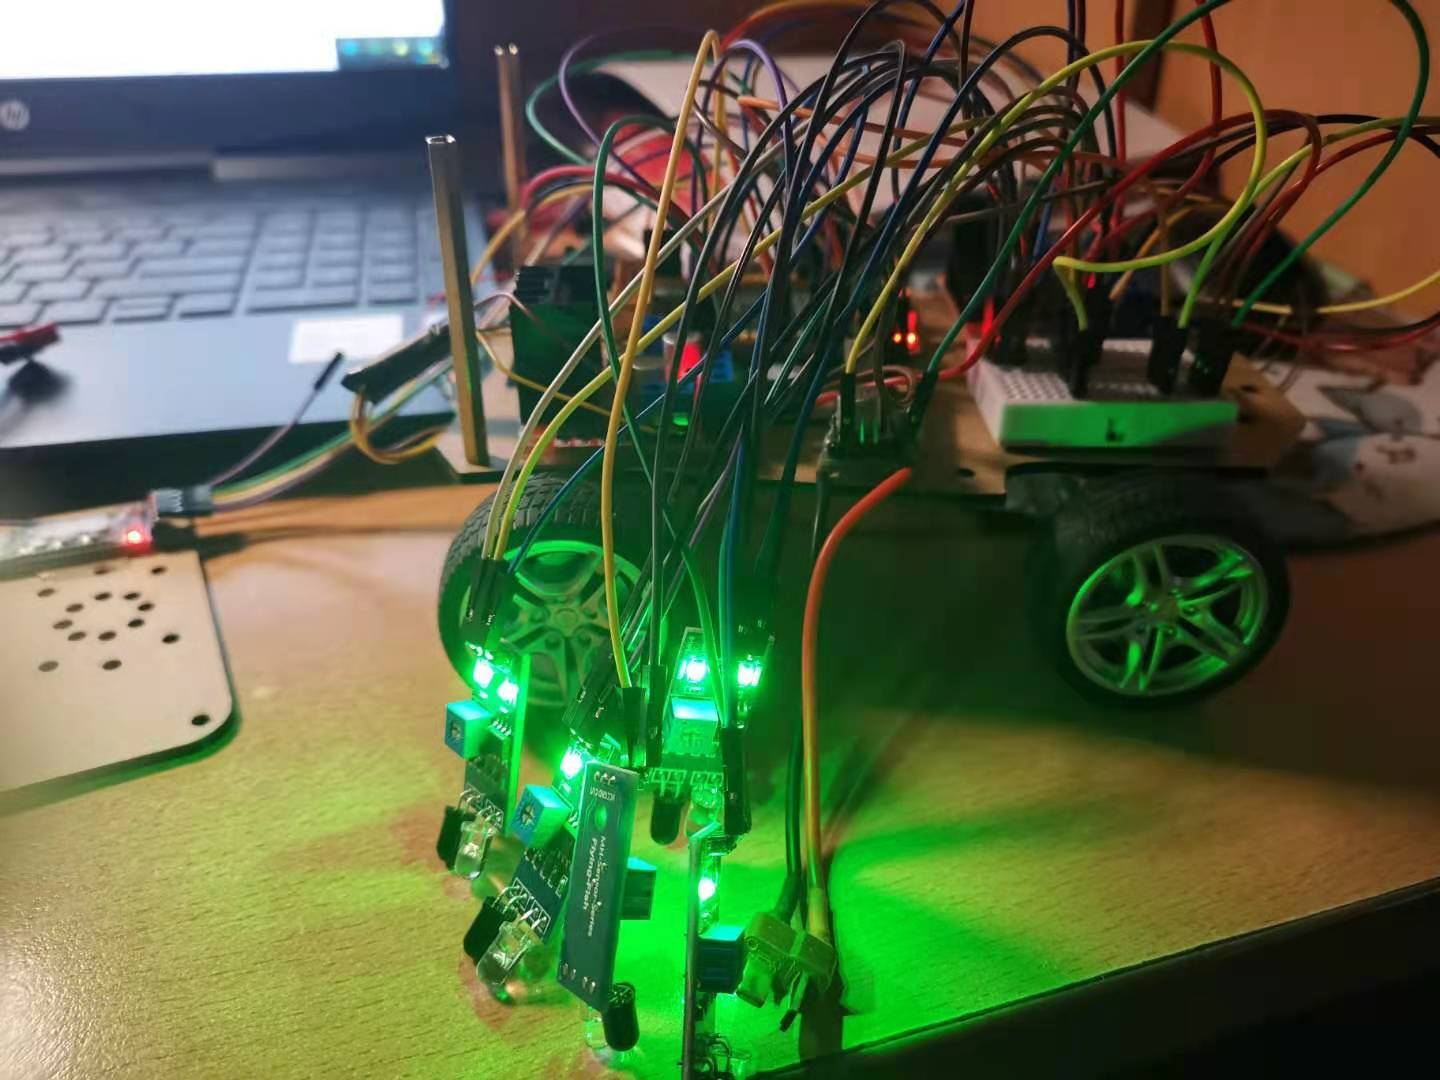
\includegraphics[width=0.75\textwidth]{1.jpg}
\end{figure}
\begin{figure}[H]
\centering
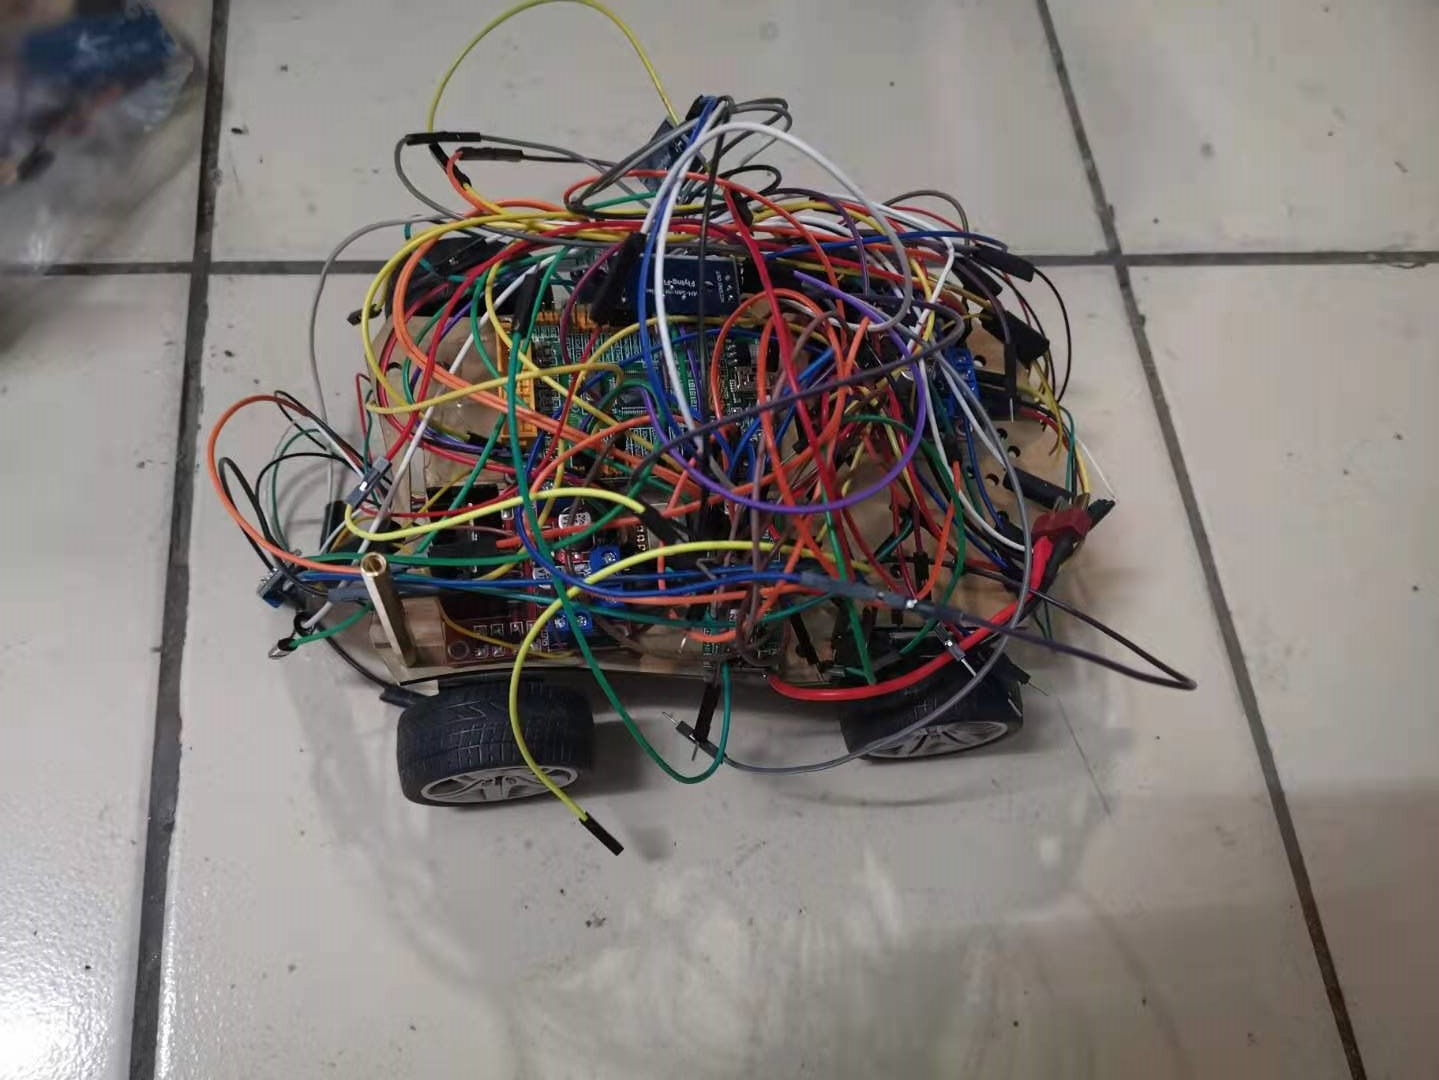
\includegraphics[width=0.65\textwidth]{2.jpg}
\end{figure}
\begin{figure}[H]
\centering
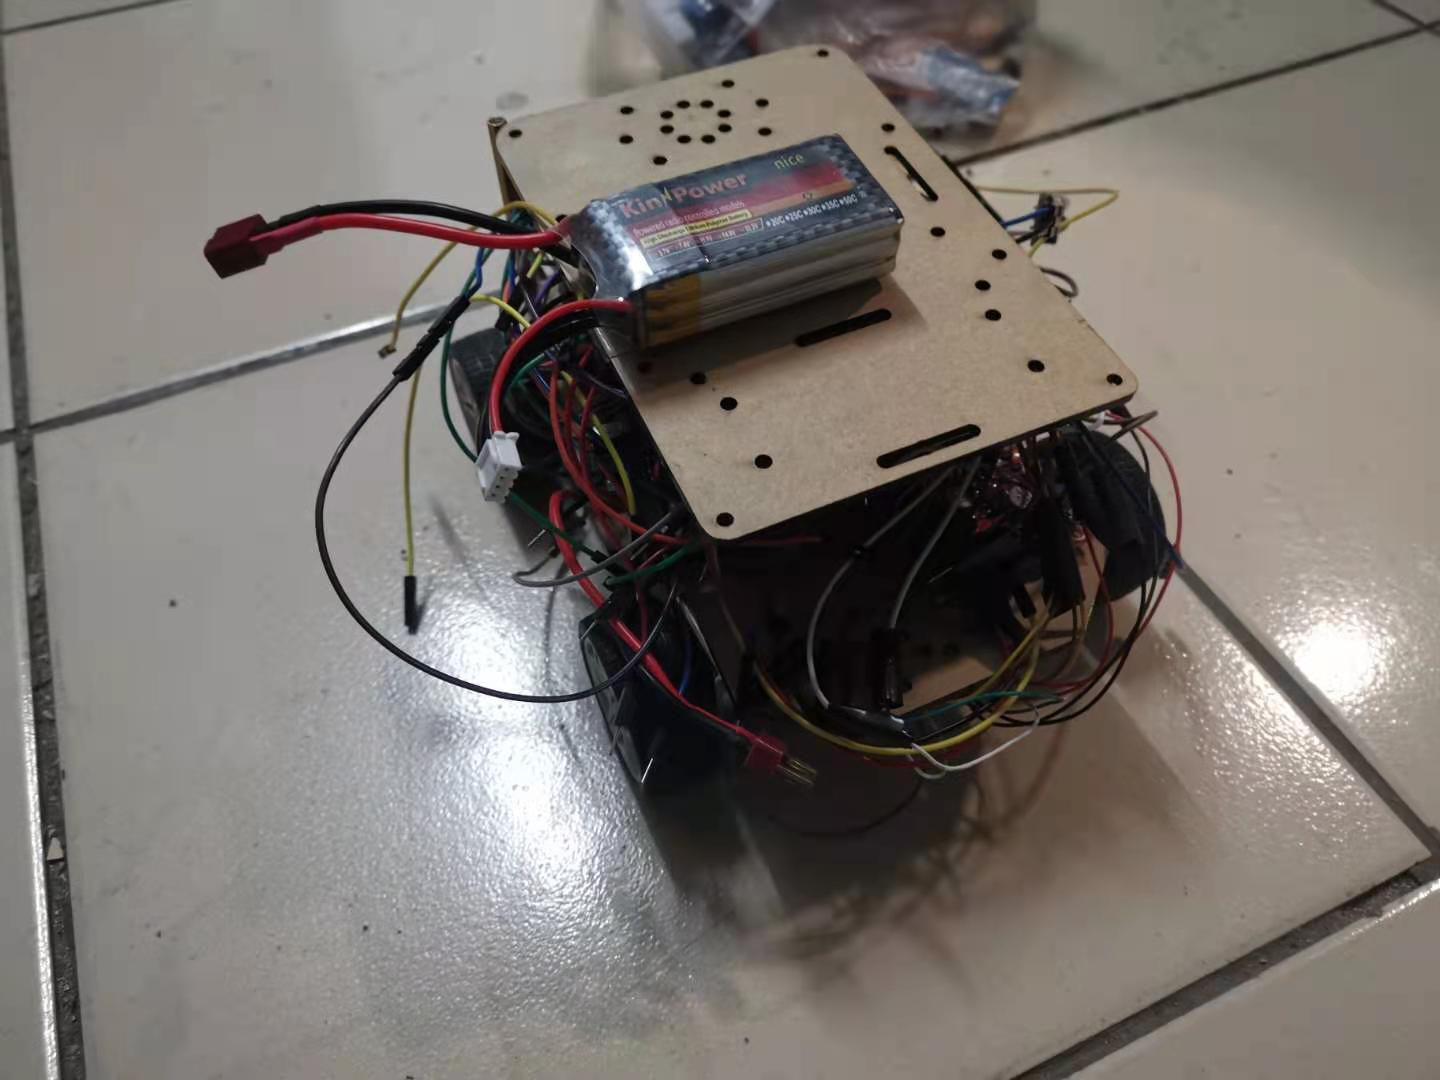
\includegraphics[width=0.8\textwidth]{3.jpg}
\end{figure}
\begin{figure}[H]
\centering
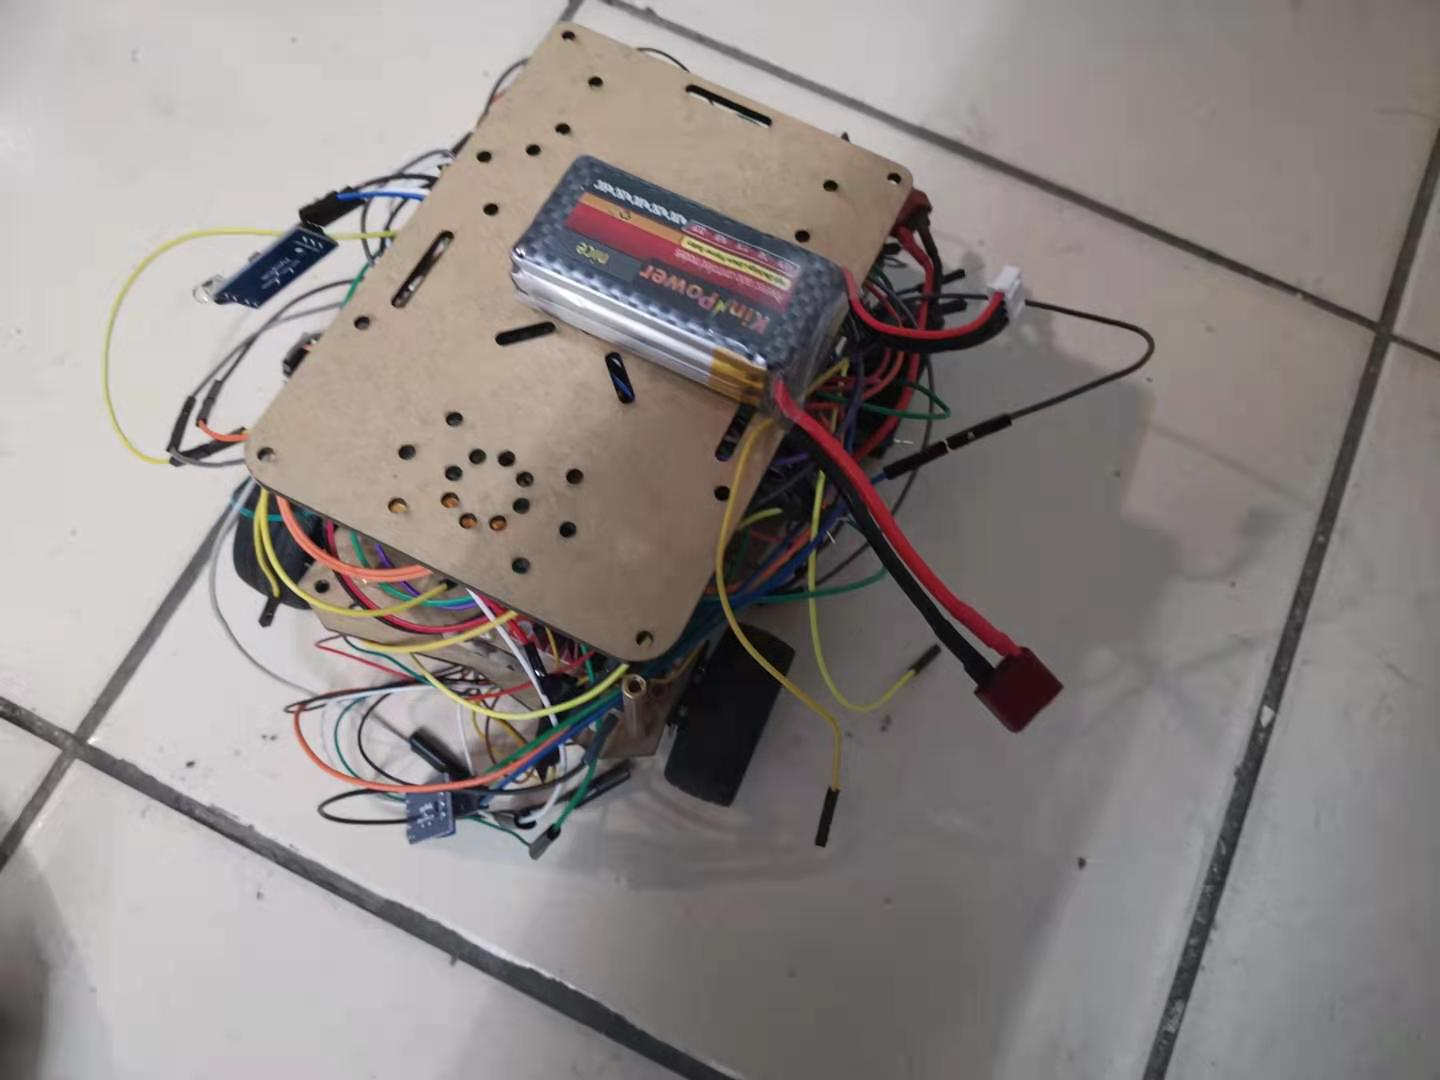
\includegraphics[width=0.8\textwidth]{4.jpg}
\end{figure}
\begin{thebibliography}{123456} 
\bibitem{ref1}《小型迷宫实现---迷宫算法(递归回溯法)》.fern$\_$girl.2017-04-24.
\bibitem{ref2}《STM32CubeMX 项目配置窗口介绍》.Brendon$\_$Tan.2020-08-09.
\bibitem{ref3}《CubeMX配置FreeRTOS跑多线程任务》.linzs.online.2019-08-30.
\bibitem{ref4}《用STM32F103读取JY62的数据》.Fred$\_$1986.2020-08-07.
\end{thebibliography}


\end{document}
